\documentclass[12pt,a4paper]{article}

\input{../../preamble_files/packages}
\input{../../preamble_files/scriptr}
\input{../../preamble_files/siunits}
\input{../../preamble_files/vectors}
\input{../../preamble_files/figures}
\input{../../preamble_files/references}
\input{../../preamble_files/empheq}

\pagestyle{fancy}
\lhead{Richard Whitehill}
\chead{PHYS 631 -- HW U}
\rhead{04/26/22}
\cfoot{\thepage \hspace{1pt} of \pageref{LastPage}}

\newcommand{\prob}[2]{\textbf{#1)} #2}

\setlength{\parskip}{\baselineskip}
\setlength{\parindent}{0pt}

\begin{document}

\prob{6.7}{
An infinitely long circular cylinder carries a uniform magnetization $\va{M}$ parallel to its axis.
Find the magnetic field (due to $\va{M}$ inside and outside the cylinder.
}

The magnetization is $\va{M} = M\zhat$, which gives the following bound current densities:
\begin{align*}
    \va{J}_{b} &= \curl{\va{M}} = 0 \\
    \va{K}_{b} &= \va{M} \cross \shat = M \phihat
.\end{align*}

This is essentially a solenoid, and we can write down the magnetic field simply using $nI = M$, giving
\begin{eqbox}
    \va{B} = \mu_{0} \va{M}
\end{eqbox}

Notice that the field is constant along the axis of the cylinder inside and zero outside the cylinder.

\prob{6.9}{
A short circular cylinder of radius $a$ and length $L$ carries a ``frozen-in'' uniform magnetization $\va{M}$ parallel to its axis.
Find the bound current, and sketch the magnetic field of the cylinder. 
(Make three sketches: one for $L \gg a$, one for $L \ll a$, and one for $L \approx a$.)
Compare this \textbf{bar magnet} with the bar electret of Prob. 4.11.
}

In this case, the current densities are the same.
Notice that there is none on the caps since the normal vector and magnetization are parallel.

\begin{figure}[H]
   \begin{center}
       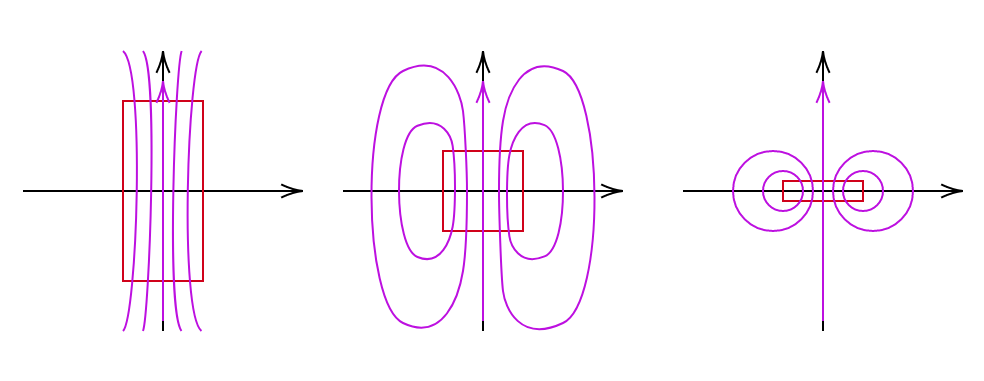
\includegraphics[scale=0.45]{./fig1.png}
   \end{center} 
\end{figure}

The left figure is the field when $L \gg a$, the center is for $L \approx a$, and the right is for $L \ll a$.
Notice that for $L \gg a$, we essentially recover the constant field of a solenoid with some fringe field behavior at the caps of the solenoid.
For $L \approx a$, the field is somewhat uniform in the center but circles around the cylinder with a nonvanishing (non-negligible) field outside the cylinder, and lastly, for $L \ll a$ we essentially have the field of a current loop.

Recall that for the bar electret we have the following cases.
\begin{enumerate}
    \item $L \gg a$: The electric field is that of a physical dipole.
    \item $L \approx a$: The electric field and magnetic fields are similar outside the cylinder, but inside they point opposite each other if the magnetization and polarization point in the same direction.
    \item $ L \ll a$: The electric field is essentially that of a parallel plate capacitor.
\end{enumerate}

\end{document}
